\documentclass[12pt]{beamer}
\usetheme{Warsaw}

\usepackage[utf8]{inputenc}
\usepackage[T1]{fontenc}
\usepackage{amsmath}
\usepackage{amsfonts}
\usepackage{amssymb}
\usepackage{graphicx}

\author{Kelompok 7}
\title{Simulasi Sistem Penataan Wi-Fi dengan Algoritma Genetika}
\logo{logo}
\institute{Sarjana Teknik Informatika Universitas Telkom}
\date{\today}
\subject{Pemodelan Sistem}
%\setbeamercovered{transparent}
%\setbeamertemplate{navigation symbols}{}

\begin{document}
	\maketitle
	
	\begin{frame}
		\frametitle{Latar Belakang}
		\begin{itemize}
			\item Wi-Fi sudah sangat umum dan dibutuhkan.
			\item Penataan AP (\emph{Access Point }) Wi-Fi masih banyak yang \emph{asal}.
			\item Instalasi langsung butuh dana besar (perangkat, sumber daya).
		\end{itemize}
	\end{frame}
	
	\begin{frame}
		\frametitle{Rumusan Masalah}
		\begin{enumerate}
			\item Bagaimanakah sistem penataan Wi-Fi yang baik agar mendapatkan wilayah jangkauan yang optimal di lingkungan nyata?
			\item Bagaimanakah menentukan sistem penataan Wi-Fi yang optimal dengan menggunakan algoritma genetika?
		\end{enumerate}
	\end{frame}
	
	\begin{frame}
		\frametitle{Tujuan}
		\begin{enumerate}
			\item Mengimplementasikan sistem penataan Wi-Fi yang optimal pada lingkungan nyata.
			\item Mengimplementasikan dan menganalisa penerapan algoritma genetika dalam menentukan sistem penataan Wi-Fi.
		\end{enumerate}
	\end{frame}
	
	\begin{frame}
		\frametitle{Batasan Masalah}
		\begin{enumerate}
			\item Dengan banyaknya jenis perangkat AP, dalam penelitian ini digunakan TP-Link TL-WR741ND 802.11b/g/n dengan antena 5dBi Omni Directional.
			\item Lokasi penelitian terbatas pada Gedung B lantai dasar di Fakultas Teknik Universitas Telkom.
			\item Material bangunan dan cuaca tidak berpengaruh.
			\item Level daya terima diukur dengan menggunakan Kismet.
			\item Jika terdapat AP yang berdekatan, dipastikan bekerja pada kanal yang berbeda.
			\item Data letak AP yang ada di gedung B merupakan data masukan awal pada simulasi. Data ini berupa koordinat dalam sumbu X,Y berbeda.
			\item Solusi optimum dinilai dari daya jangkau tertinggi, terutama di titik kritis lokasi pengujian seperti square tengah, dan sepanjang koridor sekitar kelas.
		\end{enumerate}
	\end{frame}
	
	
	\begin{frame}
		\frametitle{Metodologi}
		\begin{enumerate}
			\item Studi Literatur
			\item Pengumpulan Data
			\item Perancangan dan Implementasi
			\item Pengujian dan Analisis
			\item Penyusunan Laporan Akhir
		\end{enumerate}
	\end{frame}
	
	\begin{frame}
		\frametitle{Pengujian}
		\begin{itemize}
			\item Dilakukan pada matriks berukuran $80 x 30$
			\item Menggunakan algoritma genetika untuk optimasi
		\end{itemize}
		\framesubtitle{Tabel Hasil Pengujian}
		\begin{table}
			\centering
			\begin{tabular}{|c|c|}
				\hline \textbf{\emph{Test Case}} & \textbf{\emph{Fitness}} \\ 
				\hline 1 & 0.93 \\ 
				\hline 2 & 0.98 \\ 
				\hline 3 & 0.92 \\ 
				\hline 4 & 0.91 \\ 
				\hline 5 & 0.90 \\ 
				\hline 6 & 0.92 \\ 
				\hline 7 & 0.96 \\ 
				\hline 8 & 0.95 \\ 
				\hline 9 & 0.93 \\ 
				\hline 10 & 0.93 \\ 
				\hline 
			\end{tabular}
			\caption{Data hasil pengujian dengan AG}
			\label{tab:1}
		\end{table}
	\end{frame}
	
	\begin{frame}
		\frametitle{Analisis}
		\framesubtitle{Individu A}
		\begin{figure}[t]
		\centering
		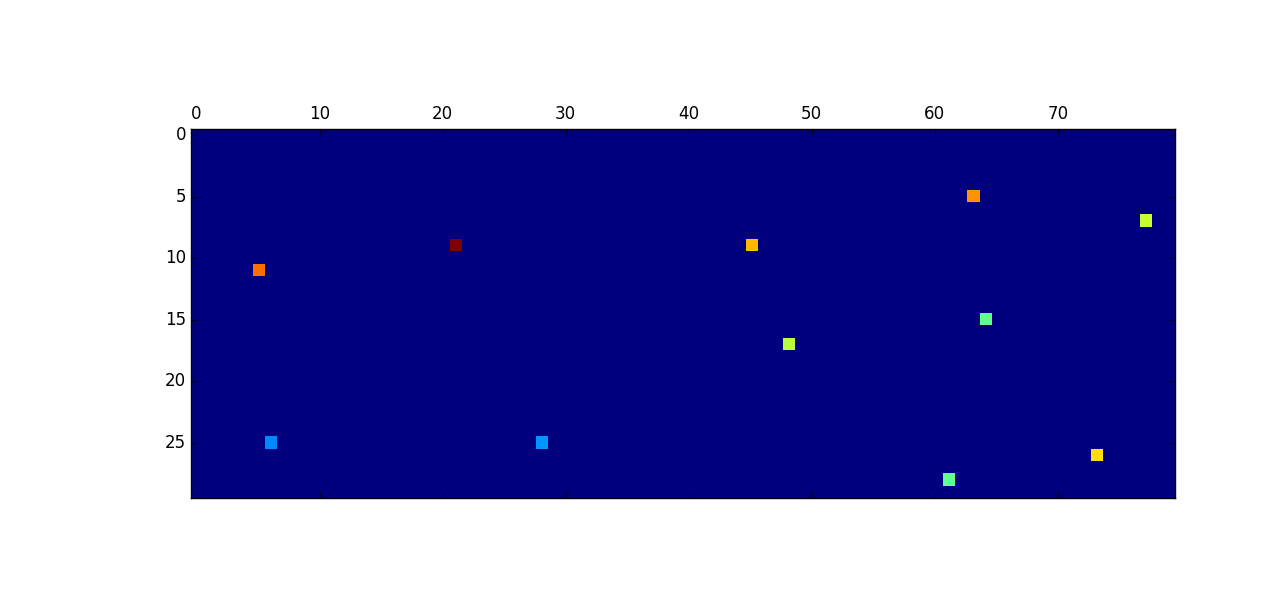
\includegraphics[width=0.5\linewidth]{apLoc_02}
		\caption{Lokasi AP individu A}
		\label{fig:apLoc_02}
		\end{figure}
		\begin{figure}[t]
			\centering
			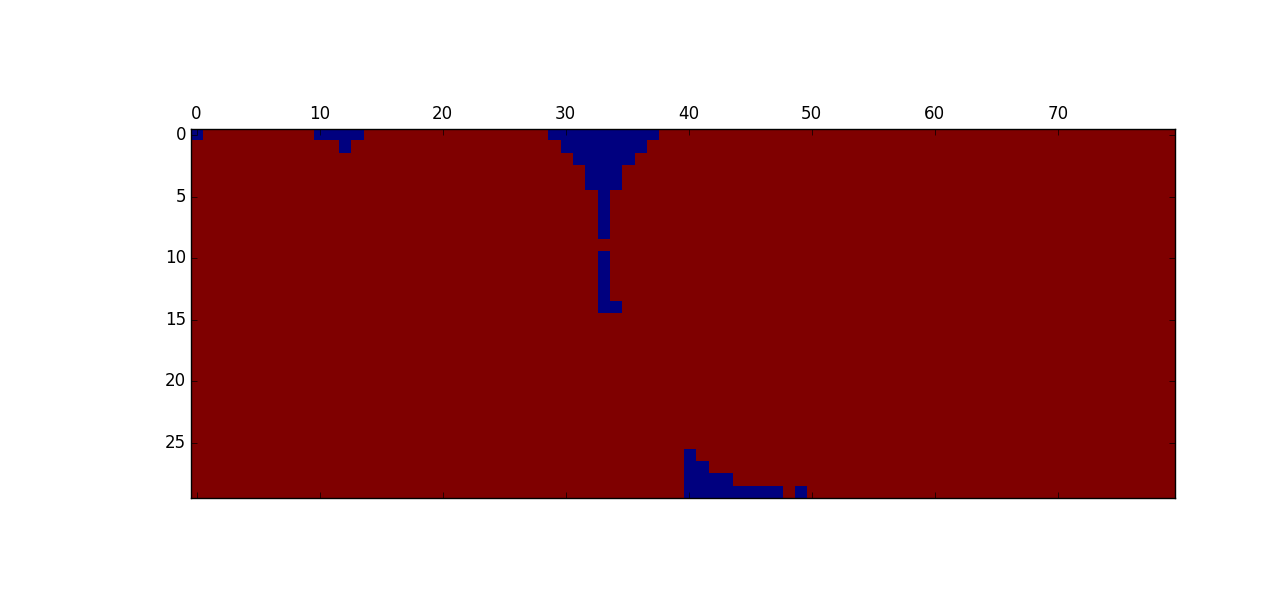
\includegraphics[width=0.5\linewidth]{coverage_02}
			\caption{Lokasi AP individu A}
			\label{fig:coverage_02}
		\end{figure}
	\end{frame}

	\begin{frame}
		\frametitle{Analisis}
		\framesubtitle{Individu B}
		\begin{figure}[t]
			\centering
			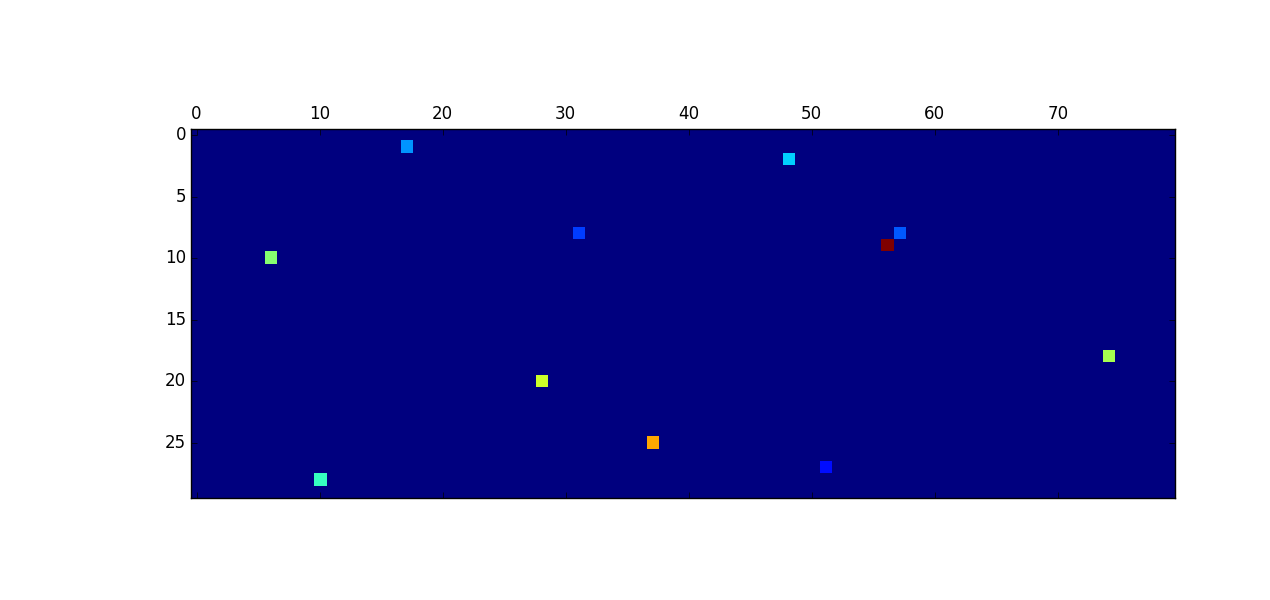
\includegraphics[width=0.5\linewidth]{apLoc_05}
			\caption{Lokasi AP individu B}
			\label{fig:apLoc_05}
		\end{figure}
		\begin{figure}[t]
			\centering
			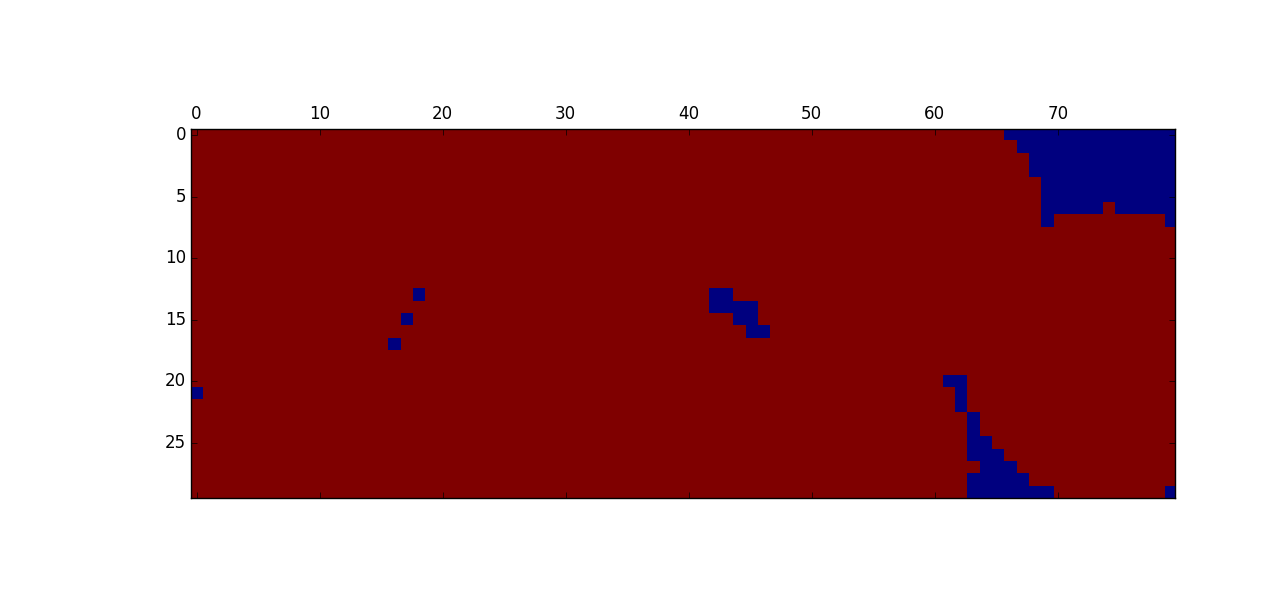
\includegraphics[width=0.5\linewidth]{coverage_05}
			\caption{Lokasi AP individu B}
			\label{fig:coverage_05}
		\end{figure}
	\end{frame}
	
	\begin{frame}
		\frametitle{Kesimpulan}
		\begin{itemize}
			\item Individu A paling optimal jika ditinjau dari nilai \emph{fitness} yang dimiliki.
			\item Individu B paling optimal jika ditinjau dari aplikasinya di lingkungan nyata. Karena, pada individu B titik kritis di Gedung B masih cukup tertutupi, sementara di bagian sisi ujung (toilet) tidak ter-\emph{cover}.
			\item Individu A kurang cocok diimplementasikan pada lingkungan nyata karena terdapat \emph{blank spot} pada titik krisis di Gedung B, yaitu bagian tengah yang notabenenya ramai pengguna.
		\end{itemize}
	\end{frame}
	
	\begin{frame}
		\frametitle{Saran}
		\begin{itemize}
			\item Perlu kajian lanjut.
			\item Libatkan parameter material dan cuaca, serta yang masih menjadi batasan masalah.
			\item Pengembangan AG
				\begin{itemize}
					\item Metode \emph{crossover}
					\item Fungsi acak peletakan AP
					\item Peletakan AP berdasar AP sebelumnya
				\end{itemize}
		\end{itemize}
	\end{frame}
	\begin{frame}
		\frametitle{Daftar Pustaka}
		\nocite{*}
		\bibliographystyle{ieeetr}
		\bibliography{laporanreferensi}
	\end{frame}
\end{document}